\chapter{Probability and Randomized Algorithm}

\section{Monty Hall Problem}

ในการการเกมโชว์แห่งหนึ่ง มีประตูอยู่ทั้งหมดสามประตู ด้านหลังของทั้งสามประตูมีของรางวัลซ่อนอยู่ โดยจะมี\emph{แพะ} อยู่สองตัว กับรถยนต์หนึ่งคัน เมื่อเกมเริ่ม ผู้เข้าร่วมเกมโชว์จะต้องเลือกประตูในดวงใจมาก่อนหนึ่งบาน (ที่อยากเปิด) แต่ยังไม่เปิด หลังจากนั้นพิธีกรจะทำการเปิดประตูขึ้นมาหนึ่งบาน โดยรับประกันว่าประตูที่เปิดออกมาเป็นแพะอย่างแน่นอน

หลังจากนั้นพิธีกรจะให้ผู้ร่วมเกมโชว์เลือก ระหว่างจะเลือกประตูเดิมที่เลือกอยู่ หรือจะสลับไปเลือกอีกประตู หลังจากผู้ร่วมเกมตัดสินใจแล้ว พิธีกรจะทำการเปิดประตูที่ผู้ร่วมเกมเลือกไว้ แล้วผู้ร่วมเกมโชว์ก็จะได้รับรางวัลเป็นของที่อยู่หลังประตูนั้น (แพะ หรือรถยนต์)

\begin{figure}[htbp]
    \centering
    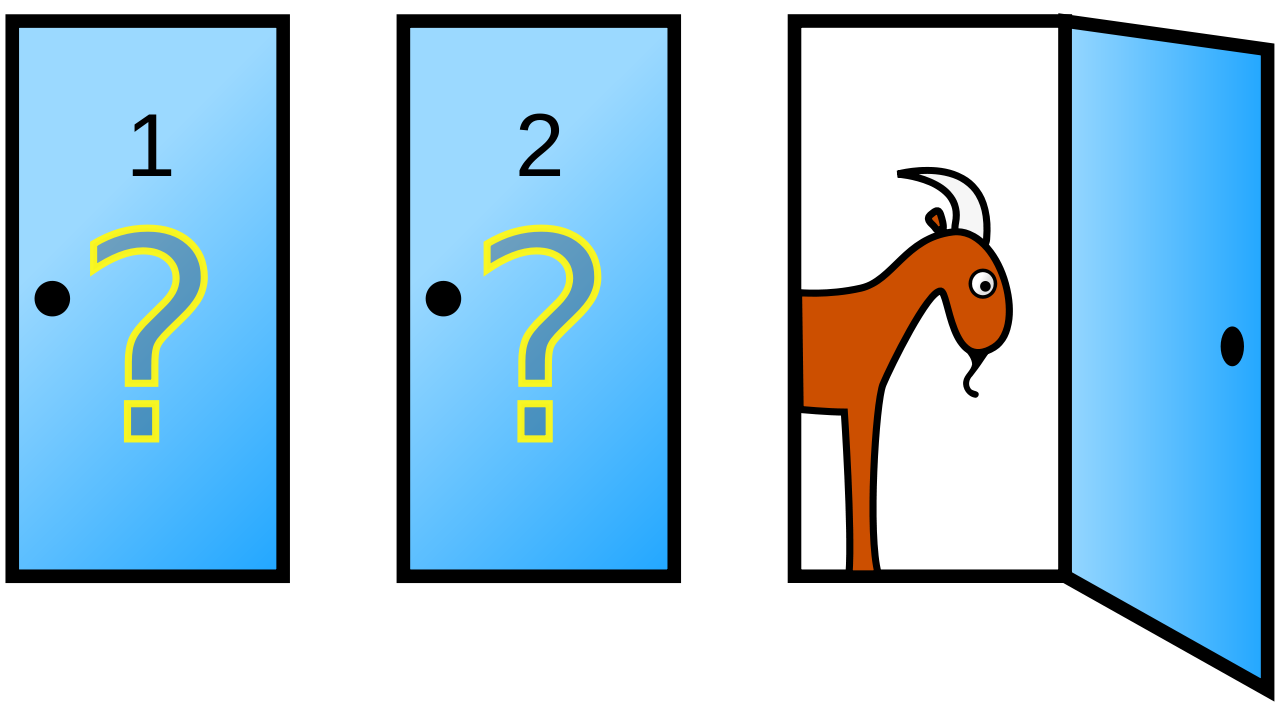
\includegraphics[width=8cm]{chapters/montyhall.png}
    \caption{ภาพแสดงการเปิดประตูไปเจอแพะ}
    \label{fig:montyhall}
\end{figure}

\begin{exercise}
หากคุณเป็นผู้เข้าร่วมเกมโชว์ และอยากได้รางวัลเป็นรถยนต์ คุณจะเลือกที่จะสลับประตูที่เปิดหลังพิธีกรเปิดประตูที่เป็นแพะหรือไม่? เพราะอะไร? และการเลือกสลับนี้มีผลต่อความน่าจะเป็นของการได้รางวัลเป็นรถยนต์หรือไม่ อย่างไร? จงอธิบาย
\end{exercise}

\section{Closest Pair of Points}

ปัญหาคลาสสิกปัญหาหนึ่งที่เป็นที่นิยมคือปัญหาคู่ของจุดที่ใกล้กันมากที่สุด (Closest pair of points) ก่อนจะไปถึงปัญหานั้น เราจะพิจารณาปัญหาที่ง่ายกว่านั้นก่อน

\begin{definition}
ให้สัญลักษณ์ $\delta(S)$ แทนระยะห่างของจุดที่ใกล้กันมากที่สุดใน $S$ (กล่าวได้ว่า $\delta \colon \R \times \R \to \R$ เป็นฟังก์ชัน)
\end{definition}

\begin{exercise}
ให้ $N \in \N$ กำหนดจุด $N$ จุดบนระนาบสองมิติ ในอาเรย์ $S$ และค่า $d$ มาให้ ให้ออกแบบอัลกอริทึมที่ตรวจสอบระหว่าง $\delta(S) > d$, $\delta(S) < d$ หรือ $\delta(S) = d$ ได้ในเวลา $O(N)$ (คำใบ้: ตารางกริดบนระนาบ)
\end{exercise}

พิจารณาอัลกอริทึมต่อไปนี้ ทำการสุ่มตำแหน่ง (shuffle) บน $S$ แล้วให้ $r_i := \delta(\{S_1, \dots, S_i\})$ จะได้ $r_1, r_2, \dots, r_N \in \R$ แล้วค่อย ๆ ดำเนินการคำนวณ $r_i$ โดยเริ่มจาก $r_1 = \infty$ แล้วค่อย ๆ ใส่จุดลงไปแล้วตรวจสอบว่า $r_i < r_{i-1}$ หรือไม่ หาก $r_i < r_{i-1}$ ทำการคำนวณหาค่า $r_i$ โดยหา $r_i = \min\{||S_i - S_j|| \colon j != i\}$ ใน $O(N)$

อัลกอริทึมข้างต้นจะใช้เวลา $O(kN)$ เมื่อ $k$ แทนจำนวนครั้งที่ $r_i < r_{i-1}$

เมื่อพิจารณาอย่างละเอียด จะกล่าวได้ว่าเวลารวมที่ใช้จะเป็นสัดส่วนกับ
\[
R = 1 + \sum_{i=2}^N (1 + i X_i)
\]
เมื่อ $X_i$ เป็นตัวแปรสุ่ม ที่หาก $r_i < r_{i-1}$ แล้วจะมีค่าเป็น $1$ มิฉะนั้นจะมีค่าเป็น $0$

\begin{exercise}
จงพิสูจน์ว่า $\Pr(X_i = 1) \leq \frac{2}{i}$ สำหรับทุก $i \in \{2, \dots, N\}$
\end{exercise}

\begin{exercise}
จงพิสูจน์ว่า $\mathbb{E}[R] \leq 3n$ และสรุปผล
\end{exercise}

\section{Bloom Filter}

โครงสร้างข้อมูลแบบหนึ่งมีชื่อว่า Bloom Filter โดยสามารถทำหน้าที่ได้ดังนี้
\begin{itemize}[nosep]
    \item ใส่ค่า $x$ ลงใน Bloom Filter
    \item ตรวจสอบว่ามีค่า $x$ อยู่ใน Bloom Filter หรือไม่
\end{itemize}

โดย Bloom Filter นั้น ข้อเสียคือเวลาตรวจสอบมีโอกาสผิดพลาดแบบ false positive (ตอบว่ามีทั้ง ๆ ที่ไม่มี) ได้ แต่ว่าจะไม่มีทางตอบว่าไม่มีทั้ง ๆ ที่มี ส่วนข้อดีคือเป็นโครงสร้างที่สร้างมาเพื่อประหยัดพื้นที่

หลักการทำงานของ Bloom Filter คือ หากเราทราบว่าจะมีการใส่ค่าทั้งหมด $n$ ค่า และเราต้องการเตรียม Bloom Filter ขนาด $m$ บิต เราจะสร้างแฮชฟังก์ชันที่แตกต่างกัน $k$ ฟังก์ชันที่ส่งผลลัพธ์อย่างสุ่ม

โดยเริ่มต้น เราจะปรับให้ทุกบิตของ Bloom Filter เป็นศูนย์ก่อน ต่อมา สมมติแฮชฟังก์ชันชื่อ $h_1, h_2, \dots, h_k$ เมื่อเราต้องการใส่ค่า $x$ ลงไป เราจะทำการคำนวณ $b_1 = h_1(x), b_2 = h_2(x), \dots, b_k = h_k(x)$ แล้วปรับค่าช่องที่ $b_1, b_2, \dots, b_k$ บน Bloom Filter ให้เป็นหนึ่งให้หมด

\begin{figure}[htbp]
    \centering
    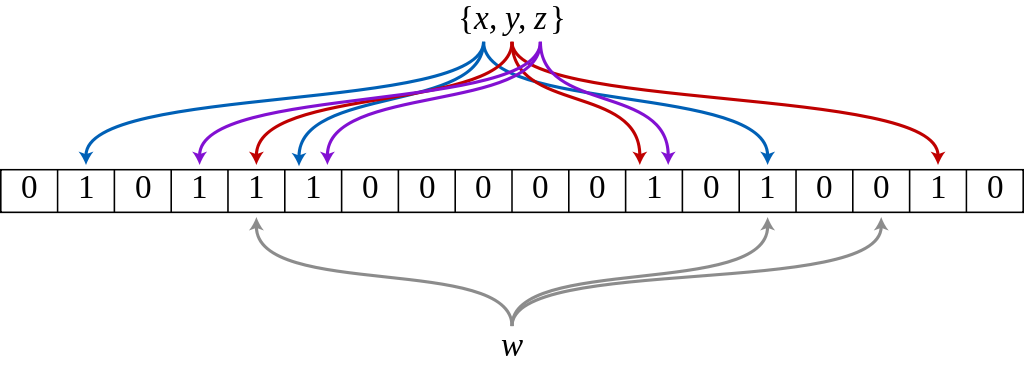
\includegraphics[width=10cm]{chapters/bloomfilter.png}
    \caption{รูปแสดงการทำงานของ Bloom Filter}
    \label{fig:bloom_filter}
\end{figure}

เมื่อมีคำถามว่ามี $x$ อยู่ในนี้หรือไม่ เราก็ทำการคำนวณ $b_1 = h_1(x), b_2 = h_2(x), \dots, b_k = h_k(x)$ เหมือนเดิม แล้วตรวจสอบว่าช่องที่ $b_1, b_2, \dots, b_k$ บน Bloom Filter นั้นเป็นหนึ่งทั้งหมดหรือไม่ หากมีช่องใดช่องหนึ่งไม่เป็นหนึ่ง เราสรุปได้ทันทีว่า $x$ ไม่อยู่ในนี้ แต่หากทุกช่องเป็น $1$ เราสรุปอะไรไม่ได้ จึงตอบได้ว่ามีความเป็นไปได้สูงที่ $x$ จะอยู่ในนี้

สมมติให้แฮชฟังก์ชันคืนค่าโดยสุ่มอย่างเท่าเทียบ (หมายถึงความน่าจะเป็นที่ $h(x) = i$ นั้นเท่ากันหมดสำหรับทุก $i$ จากทั้ง $m$ ช่อง) แสดงว่า ความน่าจะเป็นที่ $h(x)$ จะเท่ากับค่าค่าหนึ่ง มีค่าเท่ากับ $\frac{1}{m}$ 

\begin{exercise}
จงพิสูจน์ว่า หากแฮชฟังก์ชันไม่ค่อยจะเกิดการแทรกซ้อนกัน (ให้คิดเสียว่าแฮชฟังก์ชันแต่ละตัวไม่เกี่ยวข้องกัน) และ $m$ มีค่ามาก จงพิสูจน์ว่าความน่าจะเป็นที่บิตบิตหนึ่งจะยังเป็นศูนย์ หลังจากใส่ของลงไปไม่ซำ้กัน $n$ ชิ้น จะมีค่าประมาณ $e^\frac{-kn}{m}$

(คำใบ้: เนื่องจาก $\lim\limits_{m \to \infty} \left(1-\frac{1}{m}\right)^m = e$ เราจึงสามารถประมาณค่า $\left(1-\frac{1}{m}\right)^m \approx e$ ได้)
\end{exercise}

\begin{exercise}
คราวนี้ เมื่อพิจารณาการทดสอบว่า $x$ อยู่ใน Bloom Filter หรือไม่ จงพิสูจน์ว่าความน่าจะเป็นที่จะตอบผิด (ไม่อยู่แต่ตอบว่าอยู่) มีค่าประมาณ
\[
\varepsilon = (1-e^\frac{-kn}{m})^k
\]
\end{exercise}

\begin{exercise}
จงพิสูจน์ว่า หากทราบค่า $m$ และ $n$ ล่วงหน้าแล้ว ค่า $k$ ที่ดีที่สุดจะมีค่าใกล้เคียงกับ $\frac{m}{n} \ln(2)$
\end{exercise}

\begin{exercise}
หาก $k = \frac{m}{n} \ln(2)$ และ $n = 1\,000\,000$ จะต้องใช้หน่วยความจำกี่บิต (กล่่าวคือจงหาค่าของ $m$ ที่น้อยที่สุด) เพื่อที่จะมั่นใจได้ว่าความน่าจะเป็นที่จะตอบถูกมีค่าอย่างน้อย $95\%$
\end{exercise}